\documentclass[11pt,a4paper]{article}
\usepackage{fontspec}
\setmainfont[Path=fonts/,FontIndex=7,BoldFont=AvenirNext.ttc,BoldFeatures={FontIndex=2},ItalicFont=AvenirNext.ttc,ItalicFeatures={FontIndex=4},BoldItalicFont=AvenirNext.ttc,BoldItalicFeatures={FontIndex=3}]{AvenirNext.ttc}
\setsansfont[Path=fonts/,FontIndex=7,BoldFont=AvenirNext.ttc,BoldFeatures={FontIndex=2},ItalicFont=AvenirNext.ttc,ItalicFeatures={FontIndex=4},BoldItalicFont=AvenirNext.ttc,BoldItalicFeatures={FontIndex=3}]{AvenirNext.ttc}
\newfontfamily\heavy[Path=fonts/,FontIndex=2]{AvenirNext.ttc}
\setmonofont[Path=fonts/,BoldFont=JetBrainsMono-Bold.ttf,ItalicFont=JetBrainsMono-Italic.ttf,Contextuals=NoAlternate,Ligatures=NoCommon]{JetBrainsMono-Regular.ttf}
\usepackage{xcolor,graphicx,tikz,booktabs,tabularx,listings,amsmath}
\usetikzlibrary{arrows.meta,positioning}
\definecolor{paper}{HTML}{FFFFFF}
\definecolor{ink}{HTML}{252525}
\definecolor{teal}{HTML}{252525}
\definecolor{orange}{HTML}{777777}
\definecolor{wash}{HTML}{EAEAEA}
\definecolor{quiet}{HTML}{666666}
\definecolor{lightink}{HTML}{D0D0D0}
\definecolor{codepaper}{HTML}{F6F6F4}
\lstset{language=Python,basicstyle=\ttfamily\fontsize{9.5}{13}\selectfont\color{ink},keywordstyle=\bfseries\color{ink},commentstyle=\itshape\color{quiet},stringstyle=\color{ink},showstringspaces=false,columns=fullflexible,keepspaces=true,breaklines=true,breakatwhitespace=true,numbers=none,upquote=true,aboveskip=8pt,belowskip=6pt}
\hyphenpenalty=4000
\emergencystretch=3em
% The same two-line navigation and fine rule as the reference, without a candy motif.
\newcommand{\guideheader}[2]{\begin{tikzpicture}[remember picture,overlay]
\node[anchor=north west,inner sep=0,text width=176mm] at ([xshift=16mm,yshift=-7mm]current page.north west) {\fontsize{8.5}{10}\selectfont\color{quiet}#1};
\node[anchor=north west,inner sep=0,text width=176mm] at ([xshift=16mm,yshift=-11.5mm]current page.north west) {\heavy\fontsize{10}{12}\selectfont\color{ink}#2};
\draw[lightink,line width=.4pt] ([xshift=16mm,yshift=-17mm]current page.north west)--([xshift=192mm,yshift=-17mm]current page.north west);
\end{tikzpicture}}

\usepackage[a4paper,left=16mm,right=18mm,top=24mm,bottom=19mm,headheight=14pt]{geometry}
\usepackage{fancyhdr,enumitem,hyperref}
\hypersetup{colorlinks=true,linkcolor=teal,urlcolor=teal}
\setlength{\parindent}{0pt}
\setlength{\parskip}{7pt}
\setlist{nosep,leftmargin=1.4em}
\usepackage{needspace,colortbl}
\lstdefinestyle{numbered}{numbers=left,numberstyle=\ttfamily\fontsize{7.5}{13}\selectfont\color{lightink},numbersep=10pt,xleftmargin=24pt}
\pagestyle{fancy}\fancyhf{}
\fancyhead[C]{\guideheader{Lesson 3 · Mortal Kombat Tower and Array Description}{Worksheet · \nouppercase{\leftmark}}}
\fancyfoot[L]{\fontsize{8}{10}\selectfont\color{quiet}LESSON 3 / Mortal Kombat Tower and Array Description}
\fancyfoot[R]{\fontsize{9}{11}\selectfont\color{quiet}\thepage}
\renewcommand{\headrulewidth}{0pt}
\newcommand{\topic}[2]{\clearpage\markboth{#2}{}{\color{quiet}\fontsize{9}{12}\selectfont\textbf{#1}}\par{\heavy\fontsize{19}{23}\selectfont\raggedright #2\par}\vspace{5pt}}
\newcommand{\topicflow}[2]{\par\Needspace{20\baselineskip}\bigskip\markboth{#2}{}{\color{quiet}\fontsize{9}{12}\selectfont\textbf{#1}}\par{\heavy\fontsize{19}{23}\selectfont\raggedright #2\par}\vspace{5pt}}
\newcommand{\labeltext}[1]{{\color{teal}\textbf{#1}}\par}
\begin{document}\color{ink}\fontsize{10.5}{13}\selectfont
\thispagestyle{empty}\pagecolor{white}\null
\begin{tikzpicture}[remember picture,overlay]
\node[anchor=north west,inner sep=0,text width=174mm] at ([xshift=18mm,yshift=-22mm]current page.north west)
{\heavy\fontsize{9}{12}\selectfont ALGORITHMS\quad /\quad LESSON 03\quad /\quad PRINTER-FRIENDLY WORKSHEET};
\node[anchor=north west,inner sep=0,text width=174mm] at ([xshift=18mm,yshift=-39mm]current page.north west)
{\heavy\fontsize{33}{37}\selectfont\raggedright\spaceskip=.25em Mortal Kombat Tower\\and Array Description\par};
\node[anchor=north west,inner sep=0,text width=174mm] at ([xshift=18mm,yshift=-80mm]current page.north west)
{\fontsize{19}{25}\selectfont Questions, diagrams and tables.};
\node[anchor=north west,inner sep=0,text width=150mm] at ([xshift=18mm,yshift=-97mm]current page.north west)
{\fontsize{12}{16}\selectfont Try each question on paper or in the notebook.\\Use the same question IDs to check your answers.};
\node[anchor=center,inner sep=0] at ([xshift=105mm,yshift=-167mm]current page.north west)
{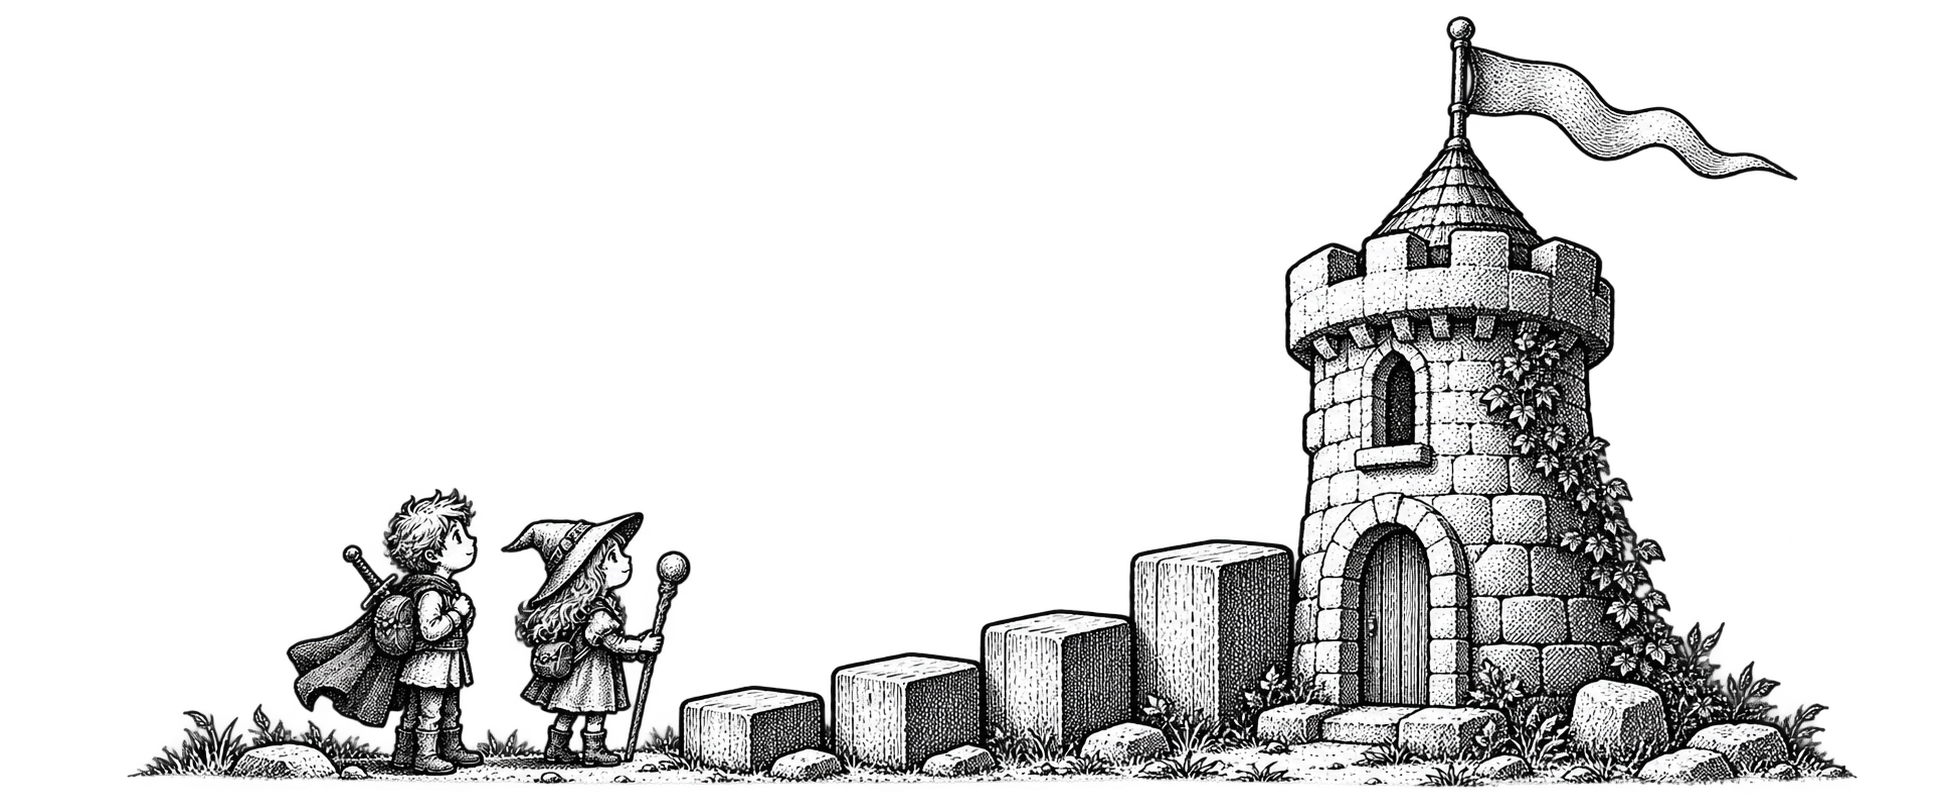
\includegraphics[width=174mm,height=94mm,keepaspectratio]{assets/cover.png}};
\node[anchor=north west,inner sep=0,text width=174mm] at ([xshift=18mm,yshift=-224mm]current page.north west)
{\fontsize{12}{16}\selectfont Understand what each step establishes\\and why it leads to the next.};
\node[anchor=west,inner sep=0] at ([xshift=18mm,yshift=-269mm]current page.north west)
{
\includegraphics[width=43mm]{assets/logo.png}};
\node[anchor=east,inner sep=0] at ([xshift=192mm,yshift=-269mm]current page.north west)
{
\includegraphics[width=62mm]{assets/julians-pathfinder-monochrome.pdf}};
\node[anchor=north west,inner sep=0,text width=174mm] at ([xshift=18mm,yshift=-244mm]current page.north west) {\fontsize{11}{14}\selectfont \href{https://colab.research.google.com/github/fifteen02/julians-pathfinder/blob/main/Lesson\%203/lesson.ipynb}{\underline{Open this lesson in Google Colab}}};
\end{tikzpicture}\clearpage
\markboth{Questions}{}\raggedbottom\setlength{\parskip}{4pt}
{\heavy\fontsize{16}{20}\selectfont Lesson 3 / Mortal Kombat Tower and Array Description\par}\medskip
\par\noindent\begin{minipage}{\linewidth}
{\heavy\fontsize{12}{15}\selectfont Tower: remember whose turn comes next\par}\medskip
\textbf{L3-01 / When one index is not enough}\par\smallskip One hard boss remains. If your friend takes the next turn, defeating it costs one point. If you take the next turn, it costs no points. Can the boss position alone identify the minimum remaining payment? What other detail must the question include?\par
\end{minipage}\par\vspace{4mm}
\par\noindent\begin{minipage}{\linewidth}
\textbf{L3-02 / Tower rules at the board}\par\smallskip Bosses are [1, 0, 1, 1]: 1 is hard and 0 is easy. Your friend starts. Players alternate turns, each defeating the next one or two bosses. Only your friend pays, one point per hard boss they defeat. Both players cooperate. Find a schedule with the smallest total payment.\par
\end{minipage}\par\vspace{4mm}
\par\noindent\begin{minipage}{\linewidth}
\textbf{L3-03 / Name the remaining question}\par\smallskip Let n be the number of bosses and i the next boss position, starting at 0. friend\_turn is True for your friend and False for you. Define cost(i, friend\_turn) in a sentence: does it include earlier payments? What should it return when i = n?\par
\end{minipage}\par\vspace{4mm}
\par\noindent\begin{minipage}{\linewidth}
\textbf{L3-04 / Compare a session and its continuation}\par\smallskip Write tower\_cached(bosses) using cached recursion. From position i, write the two legal Tower choices. How does payment depend on the player? Use these choices in your function.\par
\par\smallskip{\small\textbf{Start with:}}\par\smallskip\noindent\colorbox{codepaper}{\parbox{\dimexpr\linewidth-2\fboxsep\relax}{\small\ttfamily\raggedright def tower\_cached(bosses):\\\hspace*{2.4em}def cost(i, friend\_turn):\\\hspace*{4.8em}return None  \# Your helper goes here.\\\hspace*{2.4em}return cost(0, True)}}\par
{\small\textbf{What each function returns.}\par tower\_cached(bosses): the minimum total points paid by your friend, who starts.\par cost(i, friend\_turn): the minimum further points your friend must pay from boss i, with the indicated player next.\par }
{\small\textbf{Hints.}}\begin{itemize}\item What is the remaining cost when no bosses remain?\item On one turn, how many bosses can the player take, and who pays for them?\item After the turn, who plays next, and from which position?\end{itemize}
\end{minipage}\par\vspace{4mm}
\par\noindent\begin{minipage}{\linewidth}
\textbf{L3-05 / A table filled from the end}\par\smallskip Let friend[i] and you[i] be the least remaining cost when that player moves next at boss i. Fill both lists for [1, 0, 1, 1]. In which direction must the loop run?\par
\par\medskip \begingroup\small\setlength{\tabcolsep}{4pt}\renewcommand{\arraystretch}{1.35}\begin{tabularx}{\linewidth}{>{\raggedright\arraybackslash}X>{\raggedright\arraybackslash}X>{\raggedright\arraybackslash}X>{\raggedright\arraybackslash}X>{\raggedright\arraybackslash}X>{\raggedright\arraybackslash}X}\toprule\textbf{Next boss i} & \textbf{0} & \textbf{1} & \textbf{2} & \textbf{3} & \textbf{4}\\\midrule
friend[i] & ? & ? & ? & ? & 0\\
you[i] & ? & ? & ? & ? & 0\\
\bottomrule\end{tabularx}\endgroup\par\medskip 
\end{minipage}\par\vspace{4mm}
\par\noindent\begin{minipage}{\linewidth}
\textbf{L3-06 / Your turn: Tower boundaries}\par\smallskip Write tower\_table(bosses) using loops to fill the two lists from L3-05. Test bosses [0], [1] and [1, 1, 1]. Give a schedule for the third case. Explain why the two-boss option needs a bounds check.\par
\par\smallskip{\small\textbf{Start with:}}\par\smallskip\noindent\colorbox{codepaper}{\parbox{\dimexpr\linewidth-2\fboxsep\relax}{\small\ttfamily\raggedright def tower\_table(bosses):\\\hspace*{2.4em}return None  \# Replace with your answer.}}\par
{\small\textbf{What each function returns.}\par tower\_table(bosses): the minimum total points paid by your friend, who starts.\par }
{\small\textbf{Hints.}}\begin{itemize}\item Which positions are filled before the loop?\item In which direction must i move so that positions i + 1 and i + 2 are ready?\item Which entry is the answer, given that your friend starts?\end{itemize}
\end{minipage}\par\vspace{4mm}
\par\noindent\begin{minipage}{\linewidth}
{\heavy\fontsize{12}{15}\selectfont Arrays: remember the neighbouring value\par}\medskip
\textbf{L3-07 / Array Description: fill the gaps}\par\smallskip Values must be from 1 to 3 and neighbouring values may differ by at most 1. In [2, 0, 0, 1], zero means missing. List all valid completed arrays.\par
\end{minipage}\par\vspace{4mm}
\par\noindent\begin{minipage}{\linewidth}
\textbf{L3-08 / Position and last value}\par\smallskip Let table[i][v] count valid fillings of positions 0 through i whose value at position i is v. Position i and value v have different jobs. If v = 2, which previous values may contribute? If the input fixes position i to 1, which columns must contain 0?\par
\end{minipage}\par\vspace{4mm}
\par\noindent\begin{minipage}{\linewidth}
\textbf{L3-09 / Array recursion remembers the previous value}\par\smallskip Write array\_cached(values, m) using cached recursion for Array Description. What does the helper need besides the next position to fill?\par
\par\smallskip{\small\textbf{Start with:}}\par\smallskip\noindent\colorbox{codepaper}{\parbox{\dimexpr\linewidth-2\fboxsep\relax}{\small\ttfamily\raggedright def array\_cached(values, m):\\\hspace*{2.4em}def count(i, previous):\\\hspace*{4.8em}return None  \# Your helper goes here.\\\hspace*{2.4em}return count(0, 0)}}\par
{\small\textbf{What each function returns.}\par array\_cached(values, m): the number of valid completed arrays, modulo 1,000,000,007.\par count(i, previous): the number of valid completions from position i with the given previous value, modulo 1,000,000,007.\par }
{\small\textbf{Hints.}}\begin{itemize}\item What does count return when every position has been filled?\item Which values may position i take if the input fixes it?\item How does the previous value restrict the next value?\end{itemize}
\end{minipage}\par\vspace{4mm}
\par\noindent\begin{minipage}{\linewidth}
\textbf{L3-10 / The full array-count table}\par\smallskip For input [2, 0, 0, 1], allow values 1 to 3. Fill table[i][v]: the number of valid fillings through position i ending in value v. The first row is supplied. Explain one entry in the next row, then complete the table. Which final-row entries contribute to the total?\par
\par\medskip \begingroup\small\setlength{\tabcolsep}{4pt}\renewcommand{\arraystretch}{1.35}\begin{tabularx}{\linewidth}{>{\raggedright\arraybackslash}X>{\raggedright\arraybackslash}X>{\raggedright\arraybackslash}X>{\raggedright\arraybackslash}X>{\raggedright\arraybackslash}X}\toprule\textbf{Position} & \textbf{Given} & \textbf{v = 1} & \textbf{v = 2} & \textbf{v = 3}\\\midrule
0 & 2 & 0 & 1 & 0\\
1 & 0 & ? & ? & ?\\
2 & 0 & ? & ? & ?\\
3 & 1 & ? & ? & ?\\
\bottomrule\end{tabularx}\endgroup\par\medskip 
\end{minipage}\par\vspace{4mm}
\par\noindent\begin{minipage}{\linewidth}
\textbf{L3-11 / Keep the previous row intact}\par\smallskip Let n be the array length and m the largest allowed value. before[v] holds the count ending in v at the previous position; now[v] holds it at the current position. Why do two rows suffice? Why must we finish now before assigning before = now?\par
\end{minipage}\par\vspace{4mm}
\par\noindent\begin{minipage}{\linewidth}
\textbf{L3-12 / Your turn: an unknown prefix}\par\smallskip Write array\_rolling(values, m) using a loop and two rows. First complete [0, 0, 3] using values 1 to 3, with neighbouring values differing by at most 1: fill the table and list all valid arrays. Then write your code and test both [0, 0, 3] and [1, 3] with m = 3. Explain each result.\par
\par\smallskip{\small\textbf{Start with:}}\par\smallskip\noindent\colorbox{codepaper}{\parbox{\dimexpr\linewidth-2\fboxsep\relax}{\small\ttfamily\raggedright def array\_rolling(values, m):\\\hspace*{2.4em}return None  \# Replace with your answer.}}\par
{\small\textbf{What each function returns.}\par array\_rolling(values, m): the number of valid completed arrays, modulo 1,000,000,007.\par }
{\small\textbf{Hints.}}\begin{itemize}\item What does the first row look like, when there is no previous value?\item Which entries of the previous row can lead to value v?\item Why must the new row be built separately from the old row?\end{itemize}
\par\medskip \begingroup\small\setlength{\tabcolsep}{4pt}\renewcommand{\arraystretch}{1.35}\begin{tabularx}{\linewidth}{>{\raggedright\arraybackslash}X>{\raggedright\arraybackslash}X>{\raggedright\arraybackslash}X>{\raggedright\arraybackslash}X>{\raggedright\arraybackslash}X}\toprule\textbf{Position} & \textbf{Given} & \textbf{v = 1} & \textbf{v = 2} & \textbf{v = 3}\\\midrule
0 & 0 &  &  & \\
1 & 0 &  &  & \\
2 & 3 &  &  & \\
\bottomrule\end{tabularx}\endgroup\par\medskip 
\end{minipage}\par\vspace{4mm}
\par\noindent\begin{minipage}{\linewidth}
\textbf{L3-13 / What information changes the future?}\par\smallskip Why does Tower need the next player, while Array Description needs the previous value? What details can we forget in each problem?\par
\end{minipage}\par\vspace{4mm}
\end{document}